\section{Data path}

\begin{circuitfig}[H]
	\centering
	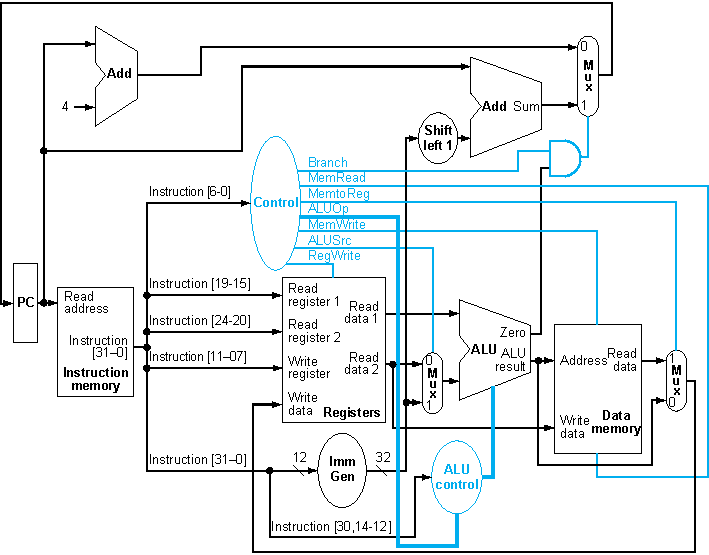
\includegraphics[width=\linewidth]{schematics/riscv.pdf}
	\caption{RISC-V processor. Το σχηματικό είναι βασισμένο στο Σχήμα 4.17 του βιβλίου Computer Organization and Design\cite{corg}.}
	\label{schematic:riscv}
\end{circuitfig}

Στην ενότητα αυτή, στο αρχείο \texttt{src/datapath.v}, υλοποιήθηκε η διαδρομή δεδομένων του επεξεργαστή του σχήματος \ref{schematic:riscv}. Οι είσοδοι του module \texttt{datapath} είναι το ρολόι, το σήμα reset, η προς εκτέλεση εντολή, το σήμα επιλογής του PC, το σήμα επιλογής του ALU source, το σήμα εγγραφής στο αρχείο καταχωρητών, το σήμα εγγραφής στο αρχείο καταχωρητών δεδομένων της κύριας μνήμης, ο κωδικός ελέγχου της ALU, το σήμα φόρτωσης της νέας διεύθυνσης του program counter και δεδομένα από την κύρια μνήμα. Όλα τα παραπάνω πλην του ρολογιού, του reset, της εντολής και του σήματος φόρτωσης του PC είναι σήματα που προέρχονται από το control unit. Οι έξοδοι του module είναι η νέα διεύθυνση του PC, το σήμα ένδειξης μηδενικού αποτελέσματος από την ALU, διεύθυνση της κύριας μνήμης, δεδομένα προς εγγραφή στην κύρια μνήμη και δεδομένα προς εγγραφή στο αρχείο καταχωρητών.\par

Οι εντολές που υποστηρίζονται από τον επεξεργαστή δίδονται στον πίνακα \ref{table:instructions}.
\begin{table}[H]
	\begin{center}
		\begin{tabular}{|r|c|c|c|c|}
			\hline
			\multirow[|r|]{3}{*}{\textbf{R-type}} & \texttt{ADD}                      & \texttt{SLT}  & \texttt{SLL}  & \texttt{SRL}  \\\cline{2-5}
			                                      & \texttt{AND}                      & \texttt{XOR}  & \texttt{OR}   & \texttt{SRA}  \\\cline{2-5}
			                                      & \multicolumn{4}{c|}{\texttt{SUB}}                                                 \\\hline\hline
			\multirow[|r|]{3}{*}{\textbf{I-type}} & \texttt{ADDI}                     & \texttt{SLTI} & \texttt{SLLI} & \texttt{SRLI} \\\cline{2-5}
			                                      & \texttt{ANDI}                     & \texttt{XORI} & \texttt{ORI}  & \texttt{SRAI} \\\cline{2-5}
			                                      & \multicolumn{4}{c|}{\texttt{LW}}                                                  \\\hline\hline
			\textbf{S-type}                       & \multicolumn{4}{c|}{\texttt{SW}}                                                  \\\hline\hline
			\textbf{B-type}                       & \multicolumn{4}{c|}{\texttt{BEQ}}                                                 \\\hline
		\end{tabular}
		\caption{Υποσύνολο των εντολών RV32I που υποστηρίζονται από τον επεξεργαστή.}
		\label{table:instructions}
	\end{center}
\end{table}

\begin{circuitfig}[H]
	\centering
	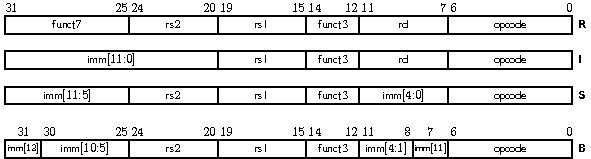
\includegraphics[width=\linewidth]{schematics/instructions.pdf}
	\caption{R, I, S και B τύποι εντολών\cite{riscv}.}
	\label{schematic:instructions}
\end{circuitfig}

Αρχικά, στο module δηλώνονται οι παράμετροι των \textsl{opcodes} των υποστηριζόμενων εντολών και τα \textsl{funct3} πεδία της κάθε εντολής.\cite{riscv}\par
Μέσω ενός \texttt{initial} block γίνεται η αρχικοποίηση του program counter. Έπειτα, με ένα \texttt{always} block το οποίο εκτελείται στις ανερχόμενες ακμές του ρολογιού υλοποιείται ο μηχανισμός του reset του program counter και ο πολυπλέκτης επιλογής της επόμενης τιμής του program counter. Συγκεκριμένα, εάν το σήμα reset είναι ενεργό η τιμή του PC επαναφέρεται στην αρχική. Διαφορετικά, εάν το σήμα φόρτωσης της νέας τιμής του PC είναι ενεργό ελέγχεται η τιμή του PCSrc (σχήμα \ref{schematic:riscv}). Εάν το PCSrc είναι ίσο με $1$ τότε η νέα τιμή του PC είναι η τρέχουσα συν το branch offset, ειδάλλως είναι η τρέχουσα προσαυξημένη κατά $4$.\par
Παρακάτω γίνεται instantiate το αρχείο καταχωρητών και υλοποιείται με ένα \texttt{always} block ο πολυπλέκτης μέσω του οποίου προκύπτει ο δεύτερος τελεσταίος της ALU. Ο πρώτος τελεσταίος είναι πάντα τα δεδομένα της πρώτης διεύθυνσης που δίνεται ως είσοδος στο αρχείο καταχωρητών. Εάν το σήμα ALUSrc είναι μηδέν, τότε ο δεύτερος τελεσταίος είναι τα δεδομένα της δεύτερης διεύθυνσης που δίνεται ως είσοδος στο αρχείο καταχωρητών. Διαφορετικά, ο δεύτερος τελεσταίος είναι το αποτέλεσμα του immediate generator του σχήματος \ref{schematic:riscv}.\par
Αμέσως μετά γίνεται instantiate η ALU και με ένα \texttt{always} block το οποίο εκτελείται όποτε αλλάζει η προς εκτέλεση εντολή, εξάγονται οι διευθύνσεις των καταχωρητών και παράγεται η σταθερή τιμή (immediate) βάσει του είδους της εντολής.\par
Για τις εντολές ολίσθησης τύπου I (\texttt{SLLI}, \texttt{SRLI} και \texttt{SRAI}) το immediate πλάτους 32 bit προκύπτει με zero extension της σταθεράς $\text{instr}[24:20]$. Για όλες τις υπόλοιπες εντολές τύπου I, συμπεριλαμβανομένης και της εντολής \texttt{LW}, το immediate πλάτους 32 bit προκύπτει με sign extension της σταθεράς $\text{instr}[31:20]$.\par
Για την εντολή \texttt{SW}. η οποία είναι τύπου S\cite{riscv}, η τιμή των 12 bit προκύπτει από τη συνένωση $\{\text{instr}[31:25],\text{instr}[11:7]\}$ η οποία, στη συνέχεια, υφίσταται επέκταση προσήμου.\par
Τέλος, η εξαγωγή του immediate για τις εντολές τύπου B είναι πιο περίπλοκη. Το immediate πλάτους 12 bit προκύπτει από τη συνένωση $\{\text{instr}[31],\text{instr}[7],\text{instr}[30:25],\text{instr}[11:8]\}$. Η τιμή αυτή υφίσταται επέκταση προσήμου και στη νέα τιμή εκτελείται ολίσθηση προς τα αριστερά κατά 1 bit, το οποίο αριθμητικά ισούται με διπλασιασμό της τιμής. Η τελική τιμή είναι το branch offset.\par
Τέλος, υλοποιείται ο πολυπλέκτης επιλογής των δεδομένων εγγραφής στο αρχείο καταχωρητών. Η διεύθυνση της κύριας μνήμης στην οποία θα εγγραφούν δεδομένα παίρνει την τιμή του αποτελέσματος της ALU. Τα δεδομένα προς εγγραφή στην κύρια μνήμη είναι τα δεδομένα του δεύτερου καταχωρητή εισόδου στο αρχείο καταχωρητών. Εάν το σήμα MemToReg είναι ενεργό, τότε τα δεδομένα προς εγγραφή στο αρχείο καταχωρητών προέρχονται από την κύρια μνήμη (εντολή \texttt{LW}). Διαφορετικά, τα δεδομένα προς εγγραφή στο αρχείο καταχωρητών προέρχονται από το αποτέλεσμα της ALU.\par